\documentclass{beamer}
\usetheme{Madrid}

\usepackage[utf8]{inputenc}
\usepackage{amsmath}
\usepackage{amsfonts}
\usepackage{amssymb}
\usepackage{graphicx}
\usepackage{xcolor}
\usepackage{tikz}

\title{CAMS Exam Preparation}
\subtitle{Complete Review of All 4 Domains (100 Slides)}
\author{Based on CAMS Candidate Handbook}
\date{}

\setbeamercovered{transparent}
\setbeamertemplate{navigation symbols}{}

\begin{document}
	
	% ============================================================
	% TITLE SLIDE
	% ============================================================
	\begin{frame}
		\titlepage
		\centering
		\textit{Domain A: 30\% | Domain B: 20\% | Domain C: 30\% | Domain D: 20\%}
	\end{frame}
	
	% ============================================================
	% DOMAIN A: UNDERSTANDING THE RISKS AND METHODS OF FINANCIAL CRIME (30%)
	% ============================================================
	
	\section{Domain A: Risks \& Methods of Financial Crime}
	
	% Subsection A.1: Definitions
	\subsection{A.1: Definitions of AML, CFT, Sanctions, Fraud, ABC, Tax Evasion}
	
	\begin{frame}{A.1.1: Money Laundering vs. Terrorist Financing}
		\begin{block}{Key Distinction (Heavily Tested)}
			\begin{itemize}
				\item \textbf{Money Laundering}: Conceals \textbf{illicit origin} of proceeds; makes funds appear legitimate
				\item \textbf{Terrorist Financing}: Funds may be \textbf{legitimate} (donations, salary); concealment objective is \textbf{intended use}, not origin
			\end{itemize}
		\end{block}
		\vspace{0.3cm}
		\textcolor{red}{\textbf{ CRITICAL:}} Standard AML controls focused on suspicious \textbf{origins} may fail to detect TF involving \textbf{clean-source funds}. TF can involve small amounts from many donors (crowdfunding).
	\end{frame}
	
	\begin{frame}{A.1.2: Predicate Offenses for Money Laundering}
		\begin{block}{FATF Recommendation 3 - Predicate Offenses}
			\begin{itemize}
				\item FATF recommends the \textbf{"all-crimes approach"} - applies to proceeds from \textbf{all serious criminal acts}
				\item \textbf{Self-laundering IS criminalized} - predicate offender can also be charged with money laundering
				\item 6AMLD harmonizes \textbf{22 predicate offenses} across EU, including tax crimes
			\end{itemize}
		\end{block}
		\vspace{0.3cm}
		\textcolor{blue}{Example:} Drug trafficker who processes own proceeds → can be charged with BOTH drug trafficking AND money laundering.
	\end{frame}
	
	\begin{frame}{A.1.3: 6AMLD - Corporate Criminal Liability}
		\begin{block}{EU Sixth Anti-Money Laundering Directive (6AMLD)}
			\begin{itemize}
				\item \textbf{Harmonizes 22 predicate offenses} across all EU member states
				\item \textbf{Introduces criminal liability for legal persons (corporations)}
				\item Corporation can be prosecuted and subject to: fines, debarment from public contracts, dissolution
				\item Does NOT require conviction of individual directors
			\end{itemize}
		\end{block}
		\textcolor{red}{\textbf{TIP:}} 6AMLD is \textbf{heavily tested} - know the difference from 5AMLD (5AMLD added VASPs and lowered prepaid card thresholds).
	\end{frame}
	
	% Subsection A.2: Financial Systems and Consequences
	\subsection{A.2: Economic and Social Consequences of ML}
	
	\begin{frame}{A.2.1: Consequences of Money Laundering}
		\begin{columns}
			\column{0.5\textwidth}
			\textbf{Economic Consequences}
			\begin{itemize}
				\item Distorts markets and asset prices
				\item Undermines legitimate private sector
				\item Loss of tax revenue
				\item Reputational damage to financial centers
			\end{itemize}
			\column{0.5\textwidth}
			\textbf{Social Consequences}
			\begin{itemize}
				\item Funds criminal enterprises (drugs, trafficking)
				\item Corruption of public officials
				\item Erodes rule of law
				\item Fuels violence and instability
			\end{itemize}
		\end{columns}
	\end{frame}
	
	\begin{frame}{A.2.2: Consequences of Indiscriminate De-Risking}
		\begin{block}{De-Risking Definition}
			Termination of entire categories of customer relationships without individual risk assessment
		\end{block}
		\textbf{Negative Consequences (Heavily Tested):}
		\begin{itemize}
			\item Legitimate businesses lose access to global financial system
			\item Drives transactions into \textbf{unregulated, informal channels} (harder to monitor)
			\item Harms financial inclusion and developing economies
			\item Contradicts the \textbf{risk-based approach}
		\end{itemize}
		\textcolor{red}{\textbf{FATF \& Wolfsberg guidance:}} Individual, documented risk assessments required - NOT blanket exclusions.
	\end{frame}
	
	% Subsection A.3: Predicate Crimes
	\subsection{A.3: Predicate Crimes Underlying Financial Crime}
	
	\begin{frame}{A.3.1: Self-Laundering and Double Jeopardy}
		\begin{block}{Self-Laundering (18 U.S.C. §1956)}
			\begin{itemize}
				\item U.S. law \textbf{DOES} criminalize self-laundering
				\item Predicate offender CAN be charged with money laundering for processing own proceeds
				\item \textbf{Double jeopardy argument fails} - each offense requires proof of different elements
			\end{itemize}
		\end{block}
		\begin{example}
			Wire fraud (predicate) + money laundering of proceeds = TWO separate crimes with distinct elements.
		\end{example}
	\end{frame}
	
	% Subsection A.4: ML/TF Manifestations Across Sectors
	\subsection{A.4: ML/TF Manifestations Across Sectors}
	
	\begin{frame}{A.4.1: Trade-Based Money Laundering (TBML)}
		\begin{block}{TBML Techniques (Heavily Tested)}
			\begin{itemize}
				\item \textbf{Over-invoicing}: Inflated prices → transfer excess value from importer to exporter
				\item \textbf{Under-invoicing}: Deflated prices → importer sells at market price, keeps surplus as "clean" funds
				\item \textbf{Phantom shipping}: No actual goods; fabricated documentation
				\item \textbf{Multiple invoicing}: Same goods invoiced multiple times
			\end{itemize}
		\end{block}
		\vspace{0.2cm}
		\textcolor{red}{\textbf{ Red flags:}} Prices significantly above/below market, shell company exporter, multiple L/C amendments, circuitous shipping routes.
	\end{frame}
	
	\begin{frame}{A.4.2: Free Trade Zone (FTZ) Vulnerabilities}
		\begin{block}{Why FTZs are High Risk}
			\begin{itemize}
				\item \textbf{Relaxed regulatory oversight}
				\item Minimal customs documentation inspections
				\item High volume of re-exported goods
				\item Opportunity for mislabeling cargo
				\item Phantom shipments
			\end{itemize}
		\end{block}
		\textbf{Red flags:} Uniform invoice values regardless of cargo, empty containers, altered bills of lading, nominee directors.
	\end{frame}
	
	\begin{frame}{A.4.3: Black Market Peso Exchange (BMPE)}
		\begin{block}{BMPE Mechanism (Heavily Tested)}
			\begin{enumerate}
				\item Narco-dollars deposited in U.S. accounts (structured)
				\item Colombian broker uses dollars to pay U.S. invoices for Colombian merchants
				\item Colombian merchant repays broker in pesos (favorable rate)
				\item \textbf{No cross-border currency movement}
			\end{enumerate}
		\end{block}
		\textbf{Key insight:} Uses drug dollars to pay legitimate commercial invoices; converts narco-dollars into domestic pesos without wire transfers.
	\end{frame}
	
	\begin{frame}{A.4.4: Black Market Peso Exchange - Diagram}
		\begin{center}
			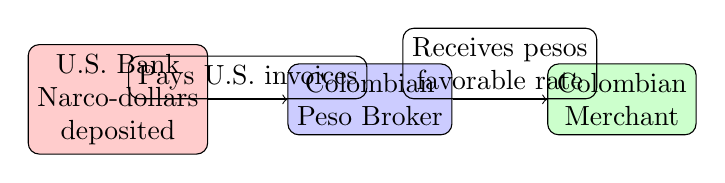
\begin{tikzpicture}[scale=0.8, every node/.style={draw, rounded corners, align=center}]
				\node[fill=red!20] (US) at (0,0) {U.S. Bank\\Narco-dollars\\deposited};
				\node[fill=blue!20] (Broker) at (4,0) {Colombian\\Peso Broker};
				\node[fill=green!20] (Merchant) at (8,0) {Colombian\\Merchant};
				\draw[->] (US) -- (Broker) node[midway, above] {Pays U.S. invoices};
				\draw[->] (Broker) -- (Merchant) node[midway, above] {Receives pesos\\favorable rate};
			\end{tikzpicture}
		\end{center}
		\textbf{No wire transfers!} The scheme uses \textbf{existing U.S. dollars} to pay legitimate invoices, avoiding cross-border movement.
	\end{frame}
	
	% Subsection A.5: Banking Sector Product Risks
	\subsection{A.5: Banking Sector Product Risks}
	
	\begin{frame}{A.5.1: Correspondent Banking Risks}
		\begin{block}{Nested Correspondent Accounts - Critical Risk}
			When a respondent bank allows third parties to route transactions through the correspondent account \textbf{without disclosure}:
			\begin{itemize}
				\item Correspondent bank loses visibility into true originators/beneficiaries
				\item Increased risk of processing for sanctioned entities
				\item Violates core KYC and correspondent banking due diligence
			\end{itemize}
		\end{block}
		\textbf{Required actions:} RFI to respondent, SAR filing, reassess relationship.
	\end{frame}
	
	\begin{frame}{A.5.2: Payable-Through Accounts (PTAs)}
		\begin{block}{PTA Obligations (U.S. Regulations)}
			\begin{itemize}
				\item Correspondent bank MUST apply CDD directly to respondent's underlying PTA accountholders
				\item Must maintain records identifying each PTA accountholder
				\item \textbf{Cannot rely solely on respondent's CDD}
			\end{itemize}
		\end{block}
		\textbf{Red flag:} Multiple sub-\$10,000 wires from different PTA accountholders to same shell company → possible structuring/money mule activity.
	\end{frame}
	
	% Subsection A.6: High-Risk Sector Banking
	\subsection{A.6: High-Risk Sector Banking}
	
	\begin{frame}{A.6.1: MSB Agent Network Risk}
		\begin{block}{MSB Principal Responsibility}
			\begin{itemize}
				\item MSB principal is \textbf{responsible for agent network compliance} under BSA
				\item Unexplained volume spikes require investigation
				\item SAR filing on agent location may be required
				\item Agent termination if compliance cannot be ensured
			\end{itemize}
		\end{block}
		\textbf{Red flag:} Agent processes 5,000\% above historical average → all transfers under \$900, same destination countries, same customer phone number.
	\end{frame}
	
	% Subsection A.7: PEP and High-Risk Customer Banking
	\subsection{A.7: PEP and High-Risk Customer Banking}
	
	\begin{frame}{A.7.1: PEP Definition and Family Members}
		\begin{block}{PEP Classification (FATF)}
			\textbf{Who qualifies as PEP:}
			\begin{itemize}
				\item Foreign heads of state/government
				\item Senior politicians, cabinet ministers
				\item Senior judicial officials
				\item Senior military officials
				\item Senior executives of state-owned enterprises
				\item \textbf{Family members and close associates} of the above
			\end{itemize}
		\end{block}
		\textcolor{red}{\textbf{Critical:}} Adult child of a foreign minister \textbf{IS a PEP family member} requiring EDD, even with no government position.
	\end{frame}
	
	\begin{frame}{A.7.2: PEP Lifecycle Management}
		\begin{block}{When a Customer Becomes a PEP (Mid-Relationship)}
			\begin{itemize}
				\item \textbf{Immediate reclassification to HIGH risk}
				\item Mandatory Enhanced Due Diligence (EDD)
				\item Re-establish and verify source of wealth AND source of funds
				\item Senior management approval to continue relationship
				\item Back-dated gap period is a control failure
			\end{itemize}
		\end{block}
		\textcolor{blue}{Example:} Customer elected to foreign cabinet → bank must re-rate immediately, NOT wait for scheduled refresh.
	\end{frame}
	
	\begin{frame}{A.7.3: Former PEP - Grace Period}
		\begin{block}{PEP Status After Retirement}
			\begin{itemize}
				\item FATF: maintain PEP status for \textbf{"reasonable period"} (min 12 months)
				\item \textbf{Risk-based decision} - consider country corruption risk, continued influence, business connections
				\item 5 years clean activity MAY justify lowering risk
				\item \textbf{Must be documented}
			\end{itemize}
		\end{block}
		\textcolor{red}{\textbf{}} No automatic rule; each decision must be documented with risk rationale.
	\end{frame}
	
	\begin{frame}{A.7.4: EDD - Source of Wealth vs. Source of Funds}
		\begin{block}{Critical Distinction (Heavily Tested)}
			\begin{itemize}
				\item \textbf{Source of Funds (SoF)}: Specific transaction being deposited (e.g., property sale contract)
				\item \textbf{Source of Wealth (SoW)}: How PEP accumulated \textbf{overall assets} (career earnings, inheritance, business)
			\end{itemize}
		\end{block}
		\textcolor{red}{\textbf{ EDD for PEPs requires BOTH.}} A lifelong civil servant with a \$4.5M Paris apartment → SoF document (sale contract) insufficient; need SoW documentation showing how property was acquired.
	\end{frame}
	
	% Subsection A.8: Other Financial Sectors
	\subsection{A.8: Other Financial Sector Risks}
	
	\begin{frame}{A.8.1: Life Insurance ML Vulnerabilities}
		\begin{block}{CDD Triggers for Life Insurance}
			\begin{itemize}
				\item Premium > USD/EUR 10,000 per year OR single premium > USD/EUR 10,000
				\item Must apply CDD to \textbf{policyholder AND beneficiary} (once designated)
			\end{itemize}
		\end{block}
		\textbf{Exploitation methods:}
		\begin{itemize}
			\item Policy loan feature = layering (convert premium to "legitimate" loan check)
			\item Cash surrender value extraction
			\item Premiums from secrecy haven jurisdictions + offshore shell company beneficiary = red flags
		\end{itemize}
	\end{frame}
	
	% Subsection A.9: MSBs, PSPs, E-commerce
	\subsection{A.9: MSBs, PSPs, E-commerce Risks}
	
	\begin{frame}{A.9.1: MSB Registration Triggers (U.S.)}
		\begin{block}{Who Must Register as MSB with FinCEN}
			\begin{itemize}
				\item Check casher cashing > \$1,000/person/day
				\item Money transmitter (any volume)
				\item Currency dealer or exchanger
				\item Issuer or seller of prepaid access
				\item Traveler's check issuer
			\end{itemize}
		\end{block}
		\textcolor{red}{\textbf{}} Grocery store cashing checks > 1,000/day without registration = BSA violation. "No ID required" policy + MSB services = ML vulnerability.
	\end{frame}
	
	% Subsection A.10: Insurance Products
	\subsection{A.10: Insurance Product Risks}
	
	\begin{frame}{A.10.1: Insurance Red Flags}
		\begin{block}{Life Insurance ML Indicators}
			\begin{itemize}
				\item Single premium payment from offshore shell company
				\item Early surrender (60 days) with proceeds to different account
				\item Policyholder is foreign PEP; beneficiary is offshore shell company
				\item Premium from secrecy haven jurisdiction
				\item Large premium relative to legitimate income
			\end{itemize}
		\end{block}
		\textbf{Layering technique:} Purchase policy → take policy loan → wire to offshore account → surrender policy.
	\end{frame}
	
	% Subsection A.11: VASPs and Cryptoassets
	\subsection{A.11: VASPs and Cryptoassets}
	
	\begin{frame}{A.11.1: FATF Travel Rule for VASPs}
		\begin{block}{Virtual Asset Travel Rule (Recommendation 16)}
			\textbf{Required information for transfers above threshold (USD/EUR 1,000):}
			\begin{itemize}
				\item Originator: name, account number/wallet ID
				\item Originator: address, national ID, or DOB (at least one)
				\item Beneficiary: name and account number/wallet ID
			\end{itemize}
		\end{block}
		\textcolor{red}{\textbf{ Receiving VASP obligations:}} Must obtain and hold info; if not provided → follow up, delay transaction, apply EDD, consider SAR.
	\end{frame}
	
	\begin{frame}{A.11.2: DeFi and AML Responsibility}
		\begin{block}{FATF DeFi Guidance - Critical Point}
			If a person/entity maintains \textbf{control or sufficient influence} over a DeFi protocol:
			\begin{itemize}
				\item Through governance token majority (>50\%) 
				\item Ability to upgrade contract code
				\item Ongoing management/control
			\end{itemize}
			\vspace{0.2cm}
			\textcolor{red}{\textbf{They may be considered a VASP}} subject to registration, KYC, transaction monitoring, and SAR filing obligations.
		\end{block}
		\textbf{Example:} 5 founders retain 68\% governance tokens and control code → likely subject to AML obligations.
	\end{frame}
	
	\begin{frame}{A.11.3: Privacy Coins and Mixers}
		\begin{block}{Anonymity-Enhanced Cryptocurrencies (AECs)}
			\textbf{Monero (XMR) risk features:}
			\begin{itemize}
				\item Ring signatures and stealth addresses obscure transaction trails
				\item Can be used with mixers/tumblers to further obfuscate
			\end{itemize}
		\end{block}
		\textbf{Red flags requiring EDD/SAR:}
		\begin{itemize}
			\item Customer deposits privacy coin → immediately exchanges → sends to non-custodial wallet → refuses to explain source
			\item Funds sent through non-regulated mixer before deposit
			\item Customer claims "privacy protection" without legitimate explanation
		\end{itemize}
	\end{frame}
	
	\begin{frame}{A.11.4: NFT Wash Trading}
		\begin{block}{NFT Wash Trading Typology}
			\begin{enumerate}
				\item Self-controlled wallets buy/sell same NFTs among themselves
				\item Prices artificially escalate through circular transactions
				\item Creates fraudulent market record
				\item Sells NFT to unwitting third party at inflated price
				\item Converts to fiat, reports as "capital gain"
			\end{enumerate}
		\end{block}
		\textbf{Exchange obligation:} File SAR based on wash trading pattern regardless of whether underlying proceeds from predicate crime.
	\end{frame}
	
	% Subsection A.12: Gaming and Gambling
	\subsection{A.12: Gaming and Gambling Risks}
	
	\begin{frame}{A.12.1: Casino Chip Washing}
		\begin{block}{Chip Washing Scheme}
			\textbf{Pattern:}
			\begin{itemize}
				\item Large cash purchase of chips (>\$10,000)
				\item Minimal gaming (45 min, \$1,500 played)
				\item Cash out rest for casino check
				\item Accepts small "gaming loss" as laundering fee
			\end{itemize}
		\end{block}
		\textbf{Obligations:} File CTR for cash-in + SAR (chip washing pattern) → combined placement and integration technique.
	\end{frame}
	
	\begin{frame}{A.12.2: Online Gaming ML}
		\begin{block}{In-Game Currency Laundering}
			\textbf{Stages:}
			\begin{enumerate}
				\item \textbf{Placement}: Purchase in-game currency with criminal cash via prepaid cards
				\item \textbf{Layering}: Distribute across multiple gamer accounts
				\item \textbf{Integration}: Sell currency peer-to-peer for PayPal, deposit to clean accounts as "gaming income"
			\end{enumerate}
		\end{block}
		\textbf{Difficulty:} Small individual transactions (\$200-\$800) fall below reporting thresholds; requires pattern recognition.
	\end{frame}
	
	% Subsection A.13: Real Estate
	\subsection{A.13: Real Estate Risks}
	
	\begin{frame}{A.13.1: FinCEN Geographic Targeting Orders (GTOs)}
		\begin{block}{GTO Requirements}
			\begin{itemize}
				\item Title insurance companies must identify \textbf{natural persons behind legal entities}
				\item All-cash purchases above threshold (\$300,000 in designated areas)
				\item Target specific metropolitan areas (Miami, LA, NYC, etc.)
				\item \textbf{Temporary} orders, renewed periodically
			\end{itemize}
		\end{block}
		\textbf{Red flags:} Recently formed LLC, IOLTA wire, registered agent refuses UBO disclosure → decline closing until UBO identified.
	\end{frame}
	
	\begin{frame}{A.13.2: Real Estate Integration}
		\begin{block}{Real Estate as Integration Vehicle}
			\textbf{Example scheme:}
			\begin{enumerate}
				\item Structured cash deposits (placement)
				\item Purchase property via anonymous LLC (layering)
				\item Rent property, report rental income on taxes (integration)
			\end{enumerate}
		\end{block}
		\textbf{Red flags for acquiring bank when property sold:}
		\begin{itemize}
			\item Rapid appreciation (e.g., \$9.5M to \$12M in 18 months)
			\item Original purchase by anonymous LLC
			\item Wire proceeds to secrecy haven account
			\item No verified source of acquisition funds
		\end{itemize}
	\end{frame}
	
	% Subsection A.14: Gatekeepers
	\subsection{A.14: Gatekeeper Risks}
	
	\begin{frame}{A.14.1: IOLTA Account Vulnerabilities}
		\begin{block}{Why IOLTA Accounts Are Dangerous}
			\begin{itemize}
				\item Banks rely on attorney's professional status
				\item \textbf{Do NOT look through} pooled account to identify individual client sub-transactions
				\item Illicit funds enter credentialed by attorney status
				\item Commingled with legitimate client funds
				\item Rapid disbursement possible
			\end{itemize}
		\end{block}
		\textbf{Red flags:} Wire from shell company to IOLTA, retainer disproportionate to transaction, no face-to-face contact, rapid disbursement to offshore.
	\end{frame}
	
	% Subsection A.15: Trusts and Company Service Providers
	\subsection{A.15: Trusts and Company Service Providers}
	
	\begin{frame}{A.15.1: Trust Beneficial Ownership}
		\begin{block}{Trust CDD Requirements (FATF)}
			Must identify and verify:
			\begin{itemize}
				\item Settlor
				\item Trustee (and its UBOs if corporate trustee)
				\item \textbf{Protector} (if has veto or replacement rights)
				\item Beneficiaries (to extent determinable)
			\end{itemize}
		\end{block}
		\textcolor{red}{\textbf{}} Protector with veto over distributions qualifies as PEP if former head of state → entire trust becomes high risk requiring EDD.
	\end{frame}
	
	\begin{frame}{A.15.2: Bearer Shares Risk}
		\begin{block}{Bearer Shares - Highest Vulnerability}
			\begin{itemize}
				\item Ownership transferred by physical delivery of certificate
				\item \textbf{NO public registry record}
				\item FATF Recommendation 24: prohibit or require immobilization with regulated custodian
			\end{itemize}
		\end{block}
		\textbf{Bank obligations:}
		\begin{itemize}
			\item Verify custodian can identify bearer share holder at all times
			\item Still need to identify UBO for CDD regardless of immobilization
			\item Decline account if custodian refuses to disclose UBO
		\end{itemize}
	\end{frame}
	
	% Subsection A.16: Accountants
	\subsection{A.16: Accountant Risks}
	
	\begin{frame}{A.16.1: Financial Statement Manipulation}
		\begin{block}{Red Flags Involving Accountants}
			\begin{itemize}
				\item Financial statements inconsistent with bank statements
				\item Unusually high "consulting fees" or "services" with no deliverables
				\item Client cannot explain discrepancy between reported income and cash flow
				\item Auditor unwilling to verify underlying records
			\end{itemize}
		\end{block}
		\textbf{Bank action:} Verify underlying records; do NOT rely solely on prepared financial statements.
	\end{frame}
	
	% Subsection A.17: Other High-Risk Sectors
	\subsection{A.17: Other High-Risk Sectors}
	
	\begin{frame}{A.17.1: Human Trafficking Financial Indicators}
		\begin{block}{Trafficking Red Flags (Heavily Tested)}
			\begin{itemize}
				\item Multiple individuals sending small payments to single controller account
				\item Controller pays utilities for multiple residential addresses
				\item Weekly cash withdrawal of 85-95\% of balance
				\item No employment contracts or payroll records
				\item Victims share same surname as controller
			\end{itemize}
		\end{block}
		\textbf{vs. Human Smuggling:} Trafficking = ongoing exploitation; Smuggling = one-time fee for illegal border crossing.
	\end{frame}
	
	\begin{frame}{A.17.2: NPO Terrorist Financing Vulnerabilities}
		\begin{block}{FATF Recommendation 8 - NPO Risks}
			\textbf{Vulnerabilities:}
			\begin{itemize}
				\item Operate in conflict zones with weak financial monitoring
				\item Enjoy public trust, receive large cash donations
				\item Limited scrutiny of fund utilization
				\item Cash withdrawals inconsistent with stated mission
			\end{itemize}
		\end{block}
		\textbf{Red flags:} Large donation from Grey List jurisdiction, rapid cash withdrawal far from HQ, transfers to conflict zone sub-NPOs where terrorists control aid.
	\end{frame}
	
	% ============================================================
	% DOMAIN B: GLOBAL AFC FRAMEWORKS, GOVERNANCE, REGULATIONS (20%)
	% ============================================================
	
	\section{Domain B: Global AFC Frameworks \& Regulations}
	
	% Subsection B.1: FATF Role and Recommendations
	\subsection{B.1: FATF Role, Function, and Recommendations}
	
	\begin{frame}{B.1.1: FATF Mutual Evaluation - Two Pillars}
		\begin{block}{Technical Compliance vs. Effectiveness}
			\begin{itemize}
				\item \textbf{Technical Compliance}: Do laws exist on paper? (40 Recommendations)
				\item \textbf{Effectiveness}: Do laws achieve intended outcomes? (11 Immediate Outcomes)
			\end{itemize}
		\end{block}
		\textcolor{red}{\textbf{ Critical:}} A country can have \textbf{perfect technical compliance} but \textbf{Low effectiveness} if:
		\begin{itemize}
			\item FIU never disseminates intelligence to law enforcement
			\item Zero ML convictions
			\item No asset forfeitures
		\end{itemize}
	\end{frame}
	
	\begin{frame}{B.1.2: FATF Immediate Outcomes (IO.1-IO.11)}
		\begin{block}{Key Immediate Outcomes (Heavily Tested)}
			\begin{itemize}
				\item \textbf{IO.1}: ML/TF risks understood and coordinated domestically
				\item \textbf{IO.6}: Financial intelligence used by competent authorities
				\item \textbf{IO.7}: ML investigated and prosecuted
				\item \textbf{IO.8}: Proceeds of crime confiscated
				\item \textbf{IO.10}: TF investigated and prosecuted
			\end{itemize}
		\end{block}
		\textbf{Evidence for IO.1:} Regular NRA that drives resource allocation, NOT just existence of laws.
	\end{frame}
	
	\begin{frame}{B.1.3: FATF Grey List vs. Black List}
		\begin{block}{Grey List - Increased Monitoring}
			\begin{itemize}
				\item Committed to action plan
				\item Apply EDD to transactions
				\item NOT automatically required to terminate relationships
				\item Individual risk assessments required
			\end{itemize}
		\end{block}
		\begin{block}{Black List - Call for Action}
			\begin{itemize}
				\item Strategic deficiencies
				\item Apply \textbf{countermeasures}
				\item May include restricting or terminating relationships
				\item FATF calls on members to act
			\end{itemize}
		\end{block}
	\end{frame}
	
	\begin{frame}{B.1.4: FATF Recommendation 16 - Wire Transfer Rule}
		\begin{block}{Required Information (Cross-border > USD 1,000)}
			\textbf{Originator:}
			\begin{itemize}
				\item Full name
				\item Account number
				\item Address, national ID, customer ID, OR DOB (at least ONE)
			\end{itemize}
			\textbf{Beneficiary:}
			\begin{itemize}
				\item Name
				\item Account number
			\end{itemize}
		\end{block}
		\textcolor{red}{\textbf{Most critical violation:}} Omitting ALL three qualifying identifiers for originator.
	\end{frame}
	
	\begin{frame}{B.1.5: FATF Recommendation 10 - CDD Triggers}
		\begin{block}{When CDD Must Be Conducted}
			\begin{enumerate}
				\item Establishing business relationship
				\item Occasional transaction above threshold (USD/EUR 15,000)
				\item Suspicion of ML/TF (regardless of amount)
				\item Doubt about veracity of previously obtained ID
			\end{enumerate}
		\end{block}
		\textbf{CDD elements:} Identify customer, verify ID, identify beneficial owner, understand purpose and intended nature, ongoing monitoring.
	\end{frame}
	
	\begin{frame}{B.1.6: FATF Recommendation 1 - Risk-Based Approach}
		\begin{block}{RBA Principles}
			\begin{itemize}
				\item Identify, assess, understand ML/TF risks
				\item Apply measures \textbf{commensurate with risks}
				\item Simplified measures where risks are lower
				\item Enhanced measures where risks are higher
				\item \textbf{NOT} zero-risk tolerance
			\end{itemize}
		\end{block}
		\textcolor{blue}{Contrast with rules-based approach:} RBA is more effective and efficient; concentrates resources on highest risks.
	\end{frame}
	
	\begin{frame}{B.1.7: FATF Recommendation 3 - Money Laundering Offense}
		\begin{block}{Key Requirements}
			\begin{itemize}
				\item Apply to \textbf{all serious predicate offenses} (all-crimes approach preferred)
				\item Apply to \textbf{self-laundering} (predicate offender can be charged)
				\item Apply regardless of whether predicate offense occurred in another jurisdiction
			\end{itemize}
		\end{block}
		\textbf{Minimum predicate offenses:} At least designated categories including drug trafficking, fraud, corruption, tax crimes.
	\end{frame}
	
	\begin{frame}{B.1.8: FATF Recommendation 5 - Terrorist Financing Offense}
		\begin{block}{TF Offense Requirements}
			\begin{itemize}
				\item Criminalize TF regardless of whether funds actually used for terrorist act
				\item \textbf{No minimum monetary threshold}
				\item Collection of funds for terrorist purposes is sufficient
				\item Standalone offense (not just covered under ML)
			\end{itemize}
		\end{block}
		\textcolor{red}{\textbf{ Deficiency:}} \$10,000 threshold violates Recommendation 5; zero convictions despite known TF activity = low effectiveness.
	\end{frame}
	
	\begin{frame}{B.1.9: FATF Recommendation 8 - NPOs}
		\begin{block}{NPO Obligations}
			\begin{itemize}
				\item Apply targeted risk-based supervision of NPOs vulnerable to TF
				\item Mechanisms to prevent NPO misuse by terrorist organizations
				\item Outreach, supervision, monitoring of cross-border transactions
			\end{itemize}
		\end{block}
		\textbf{NOT exempt:} Conflict zone NPOs are HIGH risk, not exempt. Cash withdrawal velocity mismatch with charitable mission = red flag.
	\end{frame}
	
	\begin{frame}{B.1.10: FATF Recommendation 14 - MVTS (Hawala)}
		\begin{block}{Money or Value Transfer Services}
			\begin{itemize}
				\item Must be licensed or registered
				\item Subject to AML/CFT monitoring
				\item Unlicensed providers subject to sanctions
				\item \textbf{No cultural heritage exemption} for hawala
			\end{itemize}
		\end{block}
		\textbf{Hawala risks:} Trust-based settlement, no traceable banking record, no CDD, no SAR filing.
	\end{frame}
	
	\begin{frame}{B.1.11: FATF Recommendation 15 - New Technologies}
		\begin{block}{Virtual Assets and VASPs}
			\begin{itemize}
				\item Countries must assess ML/TF risks of new technologies
				\item VASPs must be licensed or registered
				\item Subject to AML/CFT obligations (including Travel Rule)
				\item \textbf{No exemption} for DeFi if control exists
			\end{itemize}
		\end{block}
		\textbf{Applies to:} Crypto exchanges, custodian wallet providers, certain DeFi protocols with control.
	\end{frame}
	
	\begin{frame}{B.1.12: FATF Recommendation 19 - High-Risk Jurisdictions}
		\begin{block}{Response to FATF-Designated High-Risk Jurisdictions}
			\textbf{Black List (Call for Action):}
			\begin{itemize}
				\item Apply EDD to relationships and transactions
				\item Apply countermeasures (may include restricting or terminating relationships)
			\end{itemize}
			\textbf{Grey List (Increased Monitoring):}
			\begin{itemize}
				\item Apply EDD
				\item Countermeasures not automatically required
				\item Individual risk assessments
			\end{itemize}
		\end{block}
	\end{frame}
	
	\begin{frame}{B.1.13: FATF Recommendation 20 - STR Filing}
		\begin{block}{STR Timing - Critical}
			\begin{itemize}
				\item File STR \textbf{immediately upon suspicion}
				\item Regardless of transaction value
				\item \textbf{No requirement for conclusive proof}
				\item Reasonable suspicion standard
			\end{itemize}
		\end{block}
		\textcolor{red}{\textbf{}} \$2,500 suspicious transaction → MUST file STR. Cannot wait for \$10,000 threshold or conclusive evidence.
	\end{frame}
	
	\begin{frame}{B.1.14: FATF Recommendation 24 - Legal Person Transparency}
		\begin{block}{Beneficial Ownership of Legal Persons}
			\begin{itemize}
				\item Prohibit bearer shares OR require immobilization with regulated custodian
				\item Adequate, accurate, current BO information must be obtained and held
				\item Information accessible to competent authorities
			\end{itemize}
		\end{block}
		\textbf{Deficiency:} Registry not accessible to FI without court order = violation.
	\end{frame}
	
	\begin{frame}{B.1.15: FATF Recommendation 25 - Trusts}
		\begin{block}{Beneficial Ownership of Legal Arrangements}
			\begin{itemize}
				\item Trustees must hold adequate, accurate, current BO information
				\item Information accessible to competent authorities
				\item Applies to express trusts
			\end{itemize}
		\end{block}
		\textbf{Who to identify:} Settlor, trustee, protector, beneficiaries (to extent determinable).
	\end{frame}
	
	\begin{frame}{B.1.16: FATF Recommendation 26 - Supervision of FIs}
		\begin{block}{Supervisory Requirements}
			\begin{itemize}
				\item Supervisors must have adequate powers (inspect, impose sanctions)
				\item Risk-based approach to allocate resources and determine examination frequency
				\item On-site and off-site monitoring
			\end{itemize}
		\end{block}
		\textbf{Deficiency:} 5-year examination frequency for all banks regardless of risk, no penalties issued in 10 years.
	\end{frame}
	
	\begin{frame}{B.1.17: FATF Recommendation 30 - Law Enforcement}
		\begin{block}{Financial Investigation Requirements}
			\begin{itemize}
				\item LE must conduct financial investigations into ML/TF
				\item Must be able to identify, trace, initiate freezing and seizure
				\item Must have power to obtain financial records \textbf{expeditiously}
			\end{itemize}
		\end{block}
		\textbf{Deficiency:} 6-12 month delay to obtain records → undermines effectiveness.
	\end{frame}
	
	\begin{frame}{B.1.18: FATF Recommendation 32 - Cash Courier Controls}
		\begin{block}{Cross-Border Currency Declaration}
			\begin{itemize}
				\item Declaration or disclosure system for currency and bearer negotiable instruments
				\item Authority to stop/restrain couriers
				\item Sanctions for false declarations or non-disclosure
			\end{itemize}
		\end{block}
		\textbf{Deficiency:} No declaration system + intercepted couriers + no penalties = violation.
	\end{frame}
	
	% Subsection B.2: UN Role and Sanctions
	\subsection{B.2: UN Role and Sanctions Regimes}
	
	\begin{frame}{B.2.1: UNSCR 1540 - Proliferation Financing}
		\begin{block}{Proliferation Financing Red Flags}
			\begin{itemize}
				\item Export of dual-use goods to country under UNSC nuclear sanctions
				\item Payment routed through third-party intermediaries
				\item Inconsistent end-use declaration (e.g., "atmospheric research" for rad-hard ICs)
				\item Destination under UN arms embargo
			\end{itemize}
		\end{block}
		\textbf{Bank obligation:} Decline financing, file STR, notify export control authority.
	\end{frame}
	
	% Subsection B.3: Regulators, Law Enforcement, FIUs
	\subsection{B.3: Regulators, Law Enforcement, FIUs}
	
	\begin{frame}{B.3.1: Egmont Group - FIU Information Exchange}
		\begin{block}{Egmont Group Principles}
			\begin{itemize}
				\item Secure platform (Egmont Secure Web) for FIU-to-FIU exchange
				\item Information used ONLY for AML/CFT purposes
				\item Receiving FIU must maintain confidentiality
				\item \textbf{NOT a substitute for MLAT} (intelligence not automatically admissible in court)
			\end{itemize}
		\end{block}
		\textbf{MLAT vs. Egmont:} MLAT for evidence admissible in court; Egmont for intelligence sharing between FIUs.
	\end{frame}
	
	% Subsection B.4: Public/Private Sector Groups
	\subsection{B.4: Public/Private Sector Groups}
	
	\begin{frame}{B.4.1: Wolfsberg Group}
		\begin{block}{Wolfsberg Group - Key Facts}
			\begin{itemize}
				\item Private association of \textbf{13 global banks}
				\item Develops best practices and guidance (not legally binding)
				\item Focus: correspondent banking, private banking, AML/CFT
				\item CBDDQ (Correspondent Banking Due Diligence Questionnaire)
			\end{itemize}
		\end{block}
		\textbf{Most critical risk factor:} Respondent servicing unlicensed MSBs + payable-through access + 4-year audit gap.
	\end{frame}
	
	\begin{frame}{B.4.2: Basel Committee on Banking Supervision}
		\begin{block}{Basel Committee Expectations}
			\begin{itemize}
				\item AML/CFT integrated into \textbf{overall operational risk management}
				\item Across all \textbf{three lines of defense}
				\item Enterprise-Wide Risk Assessments (EWRAs) required
			\end{itemize}
		\end{block}
		\textbf{Three Lines:} 1st = business operations; 2nd = compliance; 3rd = internal audit.
	\end{frame}
	
	% Subsection B.5: Regulatory/Law Enforcement Cooperation
	\subsection{B.5: Regulatory and Law Enforcement Cooperation}
	
	\begin{frame}{B.5.1: Mutual Legal Assistance Treaties (MLATs)}
		\begin{block}{MLAT Function}
			\begin{itemize}
				\item Formal, legally binding mechanism
				\item Exchange of evidence, judicial documents
				\item Cross-border asset freezing and forfeiture
				\item Records obtained admissible in criminal proceedings
			\end{itemize}
		\end{block}
		\textbf{Process:} MLAT request from Country A to Country B's judicial authority for bank records.
	\end{frame}
	
	% Subsection B.6: Leveraging Reports from Regulators/FIUs
	\subsection{B.6: Leveraging Reports}
	
	\begin{frame}{B.6.1: National Risk Assessments (NRAs)}
		\begin{block}{Using NRA in Bank's EWRA}
			\begin{itemize}
				\item Adjust bank's EWRA to reflect national findings
				\item Enhance monitoring of identified high-risk sectors
				\item Apply additional EDD measures for sectors identified as highest risk
				\item Allocate resources proportionately
			\end{itemize}
		\end{block}
		\textbf{Example:} NRA identifies electronics imports as highest TBML risk → bank enhances monitoring of electronics import customers.
	\end{frame}
	
	% Subsection B.7: Non-Government Body Guidance
	\subsection{B.7: Non-Government Body Guidance}
	
	\begin{frame}{B.7.1: Wolfsberg CBDDQ Key Areas}
		\begin{block}{Wolfsberg CBDDQ Covers}
			\begin{enumerate}
				\item Respondent's AML/CFT policies, procedures, controls
				\item Customer base (high-risk segments: MSBs, NBFIs, foreign PEPs)
				\item Independent testing schedule and results
				\item AML program audit status
			\end{enumerate}
		\end{block}
		\textbf{NOT covered:} CEO's personal investments, office furniture, employee dress code.
	\end{frame}
	
	% Subsection B.8: National/Sectoral Risk Assessments
	\subsection{B.8: National/Sectoral Risk Assessments}
	
	\begin{frame}{B.8.1: Enterprise-Wide Risk Assessment (EWRA)}
		\begin{block}{EWRA Components}
			\begin{itemize}
				\item Inherent risk across: products, services, customer types, geographies, delivery channels
				\item Mitigating controls in place
				\item Residual risk determination
				\item Drives resource allocation
			\end{itemize}
		\end{block}
		\textbf{High residual risk (>6.0/10):} Board escalation, audit prioritization, risk mitigation plan required.
	\end{frame}
	
	% Subsection B.9: US and EU Regulations
	\subsection{B.9: US and EU Regulations}
	
	\begin{frame}{B.9.1: USA PATRIOT Act Section 311}
		\begin{block}{Section 311 - Primary ML Concern}
			\textbf{Measures that can be imposed:}
			\begin{itemize}
				\item Prohibit or condition correspondent/payable-through accounts
				\item Impose special recordkeeping/reporting requirements
			\end{itemize}
		\end{block}
		\textbf{NOT authorized:} Seize personal assets of employees, freeze all individual customer accounts.
	\end{frame}
	
	\begin{frame}{B.9.2: USA PATRIOT Act Section 313}
		\begin{block}{Shell Bank Prohibition - Absolute}
			\textbf{Shell bank definition:} Bank with NO physical presence in ANY country, NOT affiliated with regulated financial institution.
			\vspace{0.2cm}
			\textcolor{red}{\textbf{U.S. banks absolutely prohibited}} from maintaining correspondent accounts for foreign shell banks.
		\end{block}
		\textbf{No exceptions for:} G20 regulation, SAR filing, enhanced monitoring.
	\end{frame}
	
	\begin{frame}{B.9.3: USA PATRIOT Act Section 314(a)}
		\begin{block}{314(a) - Law Enforcement Requests}
			\textbf{Obligations:}
			\begin{itemize}
				\item Search accounts and transactions per FinCEN instructions
				\item Maintain confidentiality of request
				\item Report matches to law enforcement
				\item \textbf{CANNOT} freeze accounts automatically
			\end{itemize}
		\end{block}
		\textbf{Not required:} Freeze accounts, file SAR for every searched account, notify customer.
	\end{frame}
	
	\begin{frame}{B.9.4: USA PATRIOT Act Section 314(b)}
		\begin{block}{314(b) - Voluntary Information Sharing}
			\textbf{Permissible:}
			\begin{itemize}
				\item Opted-in institutions may share info about suspected ML/TF
				\item Safe harbor from liability
				\item Build complete picture across institutions
			\end{itemize}
		\end{block}
		\textbf{NOT tipping-off:} Sharing under 314(b) is explicitly permitted by law.
	\end{frame}
	
	\begin{frame}{B.9.5: USA PATRIOT Act Section 319(b)}
		\begin{block}{319(b) - Record Production}
			\begin{itemize}
				\item U.S. can demand foreign bank produce records of U.S. correspondent account
				\item If foreign bank refuses: U.S. bank may be required to terminate account
				\item Funds in account may be seized
			\end{itemize}
		\end{block}
		\textbf{Key distinction 319(a):} Forfeiture of funds in interbank accounts traceable to money laundering.
	\end{frame}
	
	\begin{frame}{B.9.6: BSA Five Pillars (31 CFR §1020.210)}
		\begin{block}{Five Required Pillars}
			\begin{enumerate}
				\item Internal controls
				\item Designated compliance officer (BSA Officer/MLRO)
				\item Ongoing employee training
				\item Independent testing
				\item Customer due diligence (including beneficial ownership)
			\end{enumerate}
		\end{block}
		\textcolor{red}{\textbf{}} All five required. CDD Rule (2016) added beneficial ownership as fifth pillar.
	\end{frame}
	
	\begin{frame}{B.9.7: FinCEN CDD Rule - Two Prongs}
		\begin{block}{Beneficial Owner Identification}
			\textbf{Ownership Prong:} Any individual owning 25\% or more of legal entity
			\vspace{0.2cm}
			\textbf{Control Prong:} At least one individual with significant managerial control (CEO, CFO, etc.)
		\end{block}
		\textbf{Aggregation required:} Direct + indirect ownership (multiply through tiers).
	\end{frame}
	
	\begin{frame}{B.9.8: SAR Safe Harbor (31 U.S.C. §5318(g))}
		\begin{block}{Safe Harbor Protections}
			\begin{itemize}
				\item Immunity from civil liability for good-faith SAR filing
				\item Immunity from liability for failure to disclose SAR to customer
				\item \textbf{Does NOT permit} using SAR as evidence in court
			\end{itemize}
		\end{block}
		\textbf{Confidentiality:} Unauthorized disclosure is criminal offense (fines + imprisonment). Retention: 5 years from filing date.
	\end{frame}
	
	% Subsection B.10: Awareness of Differing Regulatory Regimes
	\subsection{B.10: Differing Regulatory Regimes}
	
	\begin{frame}{B.10.1: Secondary Sanctions Risk}
		\begin{block}{OFAC Secondary Sanctions - Extraterritorial}
			\begin{itemize}
				\item Can target non-U.S. entities with \textbf{no U.S. nexus}
				\item Process: conduct "significant" transactions with designated sectors (Iran energy, Russia defense)
				\item Consequences: SDN listing, loss of USD correspondent access, cut off from dollar-clearing
			\end{itemize}
		\end{block}
		\textbf{EU Blocking Statute:} Provides defense in EU courts but DOES NOT prevent U.S. secondary sanctions.
	\end{frame}
	
	% Subsection B.11: Public-Private Partnerships
	\subsection{B.11: Public-Private Partnerships (PPPs)}
	
	\begin{frame}{B.11.1: PPP Purpose and Function}
		\begin{block}{Public-Private Partnership Goals}
			\begin{itemize}
				\item Improve intelligence sharing between govt and FIs
				\item Detect complex financial crime networks
				\item Share emerging typologies
				\item Help law enforcement prioritize financial intelligence
			\end{itemize}
		\end{block}
		\textbf{Does NOT replace:} SAR filing, independent testing, CDD obligations.
	\end{frame}
	
	% Subsection B.12: Private Sector Collaboration
	\subsection{B.12: Private Sector Collaboration}
	
	\begin{frame}{B.12.1: FinCEN 314(a) Search Requirements}
		\begin{block}{Search Obligations}
			\begin{itemize}
				\item Search accounts AND transactions
				\item Time period specified in request
				\item Confidentiality required
				\item Report matches (do NOT freeze accounts)
			\end{itemize}
		\end{block}
		\textbf{When search required:} Upon receipt of 314(a) request from FinCEN.
	\end{frame}
	
	% Subsection B.13: Other Laws Impacting AML (GDPR, Privacy)
	\subsection{B.13: Other Laws Impacting AML}
	
	\begin{frame}{B.13.1: GDPR vs. AML - Right to Erasure}
		\begin{block}{Resolution (GDPR Article 17(3))}
			Exception to right to erasure where retention necessary for compliance with legal obligation.
			\vspace{0.2cm}
			\textbf{AML/CFT recordkeeping obligations OVERRIDE GDPR erasure requests.}
		\end{block}
		\textbf{Also:} SAR confidentiality prohibits acknowledging existence of SAR to customer (even in GDPR response).
	\end{frame}
	
	% ============================================================
	% DOMAIN C: BUILDING AN AFC COMPLIANCE PROGRAM (30%)
	% ============================================================
	
	\section{Domain C: Building an AFC Compliance Program}
	
	% Subsection C.1: Effective Compliance Program
	\subsection{C.1: Effective Compliance Program}
	
	\begin{frame}{C.1.1: Systemic Governance Failures}
		\begin{block}{Root Causes of BSA Program Failure}
			\begin{itemize}
				\item Vacant BSA Officer position (11+ months)
				\item No independent testing independence (audit tests own designs)
				\item Missing EDD documentation (34\% of high-risk accounts)
				\item Poor SAR quality (60\% lacked sufficient detail)
				\item No program maintenance (monitoring never recalibrated in 5 years)
			\end{itemize}
		\end{block}
		\textbf{Not technology failure} → structural changes to accountability, resources, board engagement required.
	\end{frame}
	
	% Subsection C.2: Three Lines of Defense
	\subsection{C.2: Three Lines of Defense}
	
	\begin{frame}{C.2.1: Three Lines of Defense - Roles}
		\begin{block}{Correct Alignment}
			\begin{itemize}
				\item \textbf{First Line:} Business operations (relationship managers, tellers) - OWN customer relationships
				\item \textbf{Second Line:} Compliance Department, AML Officer - OVERSIGHT and guidance
				\item \textbf{Third Line:} Internal Audit - INDEPENDENT assurance to Board
			\end{itemize}
		\end{block}
		\textcolor{red}{\textbf{ Independence violation:}} Audit cannot design controls it later tests.
	\end{frame}
	
	\begin{frame}{C.2.2: Board of Directors Responsibilities}
		\begin{block}{Board AML Responsibilities}
			\begin{itemize}
				\item Approving AML compliance program and material changes
				\item Providing oversight
				\item Holding senior management accountable for AML effectiveness
				\item Receiving escalation for high residual risk
			\end{itemize}
		\end{block}
		\textbf{NOT Board responsibilities:} Filing SARs, reviewing every transaction, KYC interviews.
	\end{frame}
	
	% Subsection C.3: Risk Appetite Statement
	\subsection{C.3: Risk Appetite Statement}
	
	\begin{frame}{C.3.1: Risk Appetite Statement (RAS)}
		\begin{block}{Well-Constructed RAS}
			"Zero-tolerance for willful violations; some residual risk acceptable after controls; resources allocated proportionately to higher-risk areas."
		\end{block}
		\textbf{Key elements:}
		\begin{itemize}
			\item Acknowledges zero risk is unattainable
			\item Defines acceptable vs. unacceptable risk
			\item Guides resource allocation
			\item Board-approved
		\end{itemize}
	\end{frame}
	
	% Subsection C.4: Enterprise Risk Assessment
	\subsection{C.4: Enterprise Risk Assessment}
	
	\begin{frame}{C.4.1: Residual Risk Determination}
		\begin{block}{EWRA Process}
			Inherent Risk - Mitigating Controls = Residual Risk
		\end{block}
		\textbf{High residual risk (>6.0/10) requires:}
		\begin{itemize}
			\item Board escalation
			\item Independent audit prioritization
			\item Risk mitigation plan with timeline
		\end{itemize}
	\end{frame}
	
	% Subsection C.5: Risk-Based Approach
	\subsection{C.5: Risk-Based Approach}
	
	\begin{frame}{C.5.1: Calibrating EDD Intensity}
		\begin{block}{Risk-Proportionate EDD - Example}
			\textbf{Scenario X (Domestic PEP, \$5k salary account):}
			\begin{itemize}
				\item Verify PEP status, source of salary funds, board approval
				\item Lower intensity EDD
			\end{itemize}
			\textbf{Scenario Y (Foreign PEP, \$45M, ministry-linked funds):}
			\begin{itemize}
				\item Full source of wealth investigation
				\item Corroborated documentation
				\item Senior management sign-off
				\item Transaction-by-transaction review
			\end{itemize}
		\end{block}
	\end{frame}
	
	% Subsection C.6: Policies vs. Standards vs. Procedures
	\subsection{C.6: Policies, Standards, Procedures}
	
	\begin{frame}{C.6.1: Documentation Hierarchy}
		\begin{block}{Definitions}
			\begin{itemize}
				\item \textbf{Policies:} High-level board-approved principles
				\item \textbf{Standards:} Mandatory requirements implementing policies
				\item \textbf{Procedures:} Detailed step-by-step instructions
			\end{itemize}
		\end{block}
		\textbf{Example:} Policy = "High-risk customers require EDD" → Standard = "EDD includes SoW/SoF verification" → Procedure = Step-by-step SoW documentation guide.
	\end{frame}
	
	% Subsection C.7: Horizon Scanning
	\subsection{C.7: Horizon Scanning}
	
	\begin{frame}{C.7.1: Proactive Regulatory Monitoring}
		\begin{block}{Effective Horizon Scanning Includes}
			\begin{itemize}
				\item Regulatory proposals (pending, not just effective)
				\item FATF publications and guidance
				\item Enforcement actions against peer institutions
				\item Emerging typology reports
			\end{itemize}
		\end{block}
		\textbf{Purpose:} Adjust AML program BEFORE requirements become mandatory.
	\end{frame}
	
	% Subsection C.8: Governing Committees
	\subsection{C.8: Governing Committees}
	
	\begin{frame}{C.8.1: Documented Risk-Based Termination}
		\begin{block}{Justified Risk-Based Exit (NOT De-Risking)}
			Termination based on:
			\begin{itemize}
				\item Documented individual risk assessment (not blanket exclusion)
				\item Specific risk factors (downstream customer composition)
				\item Respondent's failure to respond to multiple RFIs
			\end{itemize}
		\end{block}
		\textbf{Defensible:} Banks not required to maintain relationships with unacceptable AML risk.
	\end{frame}
	
	% Subsection C.9: KPIs, KRIs, Board Reporting
	\subsection{C.9: KPIs, KRIs, Board Reporting}
	
	\begin{frame}{C.9.1: Effective Board Reporting Metrics}
		\begin{block}{Key Metrics for Board}
			\begin{itemize}
				\item SAR filing trends (volume, types)
				\item Alert-to-SAR conversion rates
				\item Aging of open investigations
				\item Independent testing results
				\item Regulatory exam findings
				\item Emerging typologies
			\end{itemize}
		\end{block}
		\textbf{NOT sufficient:} Total accounts opened, monthly net income, training completion counts without assessment.
	\end{frame}
	
	% Subsection C.10: FC Reporting Requirements
	\subsection{C.10: FC Reporting Requirements}
	
	\begin{frame}{C.10.1: SAR Filing Standard}
		\begin{block}{Reasonable Suspicion - NOT Conclusive Proof}
			\begin{itemize}
				\item Standard = reasonable suspicion
				\item Failure to file when standard met = regulatory risk
				\item BSA Officer can face personal liability
				\item Commercial relationship NOT a valid basis for non-filing
			\end{itemize}
		\end{block}
		\textcolor{red}{\textbf{}} "Evidence not conclusive" is NOT a valid reason to decline SAR filing.
	\end{frame}
	
	\begin{frame}{C.10.2: Alert Investigation Standards}
		\begin{block}{Material Deficiency - Unverified Assumptions}
			\begin{itemize}
				\item Cannot close alert based on unverified assumptions
				\item Must obtain supporting documentation
				\item Compare against expected activity profile
				\item Escalate if legitimate explanation cannot be documented
			\end{itemize}
		\end{block}
		\textbf{Example:} "Customer is a car dealer; cash from sales is normal" without reviewing daily sales logs = deficient.
	\end{frame}
	
	% Subsection C.11: Other Risk Management Teams
	\subsection{C.11: Other Risk Management Teams}
	
	\begin{frame}{C.11.1: Integration with Operational Risk}
		\begin{block}{Basel Committee Expectation}
			AML/CFT risk management integrated into bank's overall operational risk framework across all three lines of defense - NOT a siloed compliance function.
		\end{block}
		\textbf{Collaboration areas:}
		\begin{itemize}
			\item Cybersecurity shares threat intelligence with AML
			\item Data privacy coordinates with AML for GDPR compliance
			\item IT ensures data quality for transaction monitoring
		\end{itemize}
	\end{frame}
	
	% Subsection C.12: Controls Through Customer Lifecycle
	\subsection{C.12: Controls Through Customer Lifecycle}
	
	\begin{frame}{C.12.1: Trigger Events for Immediate KYC Refresh}
		\begin{block}{Material Change Triggers}
			\begin{itemize}
				\item Wire transfers to sanctioned jurisdictions (Syria, North Korea)
				\item Change in management/ownership
				\item New international activity not in profile
				\item Adverse media
				\item PEP designation change
			\end{itemize}
		\end{block}
		\textbf{Cannot wait for scheduled refresh (every 3 years)} - immediate out-of-cycle CDD required.
	\end{frame}
	
	% Subsection C.13: Designing/Implementing Controls
	\subsection{C.13: Designing/Implementing Controls}
	
% Subsection C.13: Designing/Implementing Controls
\subsection{C.13: Designing/Implementing Controls}

\begin{frame}{C.13.1: False Negative Risk}
	\begin{block}{77\% False Negative Rate = Material Deficiency}
		\begin{itemize}
			\item 77\% of historical SAR cases would NOT generate alerts under current thresholds
			\item NOT acceptable because alert volume is high (22k/month)
			\item Operational burden not justification for ineffective monitoring
		\end{itemize}
		\textbf{Required:} Recalibrate, document findings, remediation plan with timeline, present to board.
	\end{block}
\end{frame}  % <-- THIS CLOSING BRACE WAS MISSING!

% Subsection C.14: Role of Risk Assessment
\subsection{C.14: Role of Risk Assessment}
		% Subsection C.14: Role of Risk Assessment
		\subsection{C.14: Role of Risk Assessment}
		
		\begin{frame}{C.14.1: Multi-Dimensional Risk Matrix}
			\begin{block}{Risk Factors (rated Low/Medium/High)}
				\begin{enumerate}
					\item Customer type/PEP status
					\item Geographic risk
					\item Product/service risk
					\item Source of funds complexity
				\end{enumerate}
				\textbf{Aggregate scores:}
				\begin{itemize}
					\item 4-6: Standard CDD
					\item 7-9: Medium EDD
					\item 10-12: Full EDD + Senior Management Approval
				\end{itemize}
			\end{block}
		\end{frame}
		
		% Subsection C.15: High-Risk Scenario Controls
		\subsection{C.15: High-Risk Scenario Controls}
		
		\begin{frame}{C.15.1: Proliferation Financing Controls}
			\begin{block}{Dual-Use Goods Controls}
				\begin{itemize}
					\item End-user certification verification
					\item Trade finance documentation chain analysis
					\item Economic rationale assessment
					\item UNSC/OFAC sanctions screening
				\end{itemize}
			\end{block}
			\textbf{Red flags:} RadHard ICs + UN arms embargo destination + "atmospheric research" end-use + multi-intermediary payment.
		\end{frame}
		
		% Subsection C.16: Other Due Diligence (Employee, Third-Party)
		\subsection{C.16: Other Due Diligence}
		
		\begin{frame}{C.16.1: Insider Threat Response}
			\begin{block}{Unauthorized SAR Data Access}
				\begin{itemize}
					\item Immediate revocation of system access
					\item Escalate to HR and BSA Officer
					\item Investigate scope of unauthorized access
					\item Consider SAR filing (tipping-off, other violations)
				\end{itemize}
			\end{block}
			\textbf{Not acceptable:} Warning email only, no escalation.
		\end{frame}
		
		% Subsection C.17: Investigating Unusual Transactions
		\subsection{C.17: Investigating Unusual Transactions}
		
		\begin{frame}{C.17.1: Required Documentation}
			\begin{block}{Before Closing an Alert}
				Must obtain and review:
				\begin{itemize}
					\item Source documents (daily sales logs, title records, receipts)
					\item Compare against expected activity profile
					\item Check consistency with known customer behavior
					\item Document rationale
				\end{itemize}
			\end{block}
			\textbf{Cannot close based on:} "Customer is a dealer; cash is normal" (unverified assumption).
		\end{frame}
		
		% Subsection C.18: Documenting Investigations
		\subsection{C.18: Documenting Investigations}
		
		\begin{frame}{C.18.1: Complete Investigative File}
			\begin{block}{Required Components}
				\begin{itemize}
					\item Chronological narrative
					\item All investigative steps taken
					\item Financial data analysis
					\item Clear conclusions
					\item All supporting documentation archived
				\end{itemize}
			\end{block}
			\textbf{NOT sufficient:} "Account reviewed and deemed acceptable" with no supporting analysis.
		\end{frame}
		
		% Subsection C.19: Escalation and Offboarding
		\subsection{C.19: Escalation and Offboarding}
		
		\begin{frame}{C.19.1: Post-SAR Account Management}
			\begin{block}{SAR-Subject Account Requirements}
				\begin{itemize}
					\item Formal senior management review
					\item Documented justification for continued service
					\item BSA Officer involvement in decision
					\item Heightened ongoing monitoring
				\end{itemize}
			\end{block}
			\textbf{ Exclusion of BSA Officer = governance failure.} "Commercial importance" not a valid override.
		\end{frame}
		
		% Subsection C.20: Responding to Court Orders/Subpoenas
		\subsection{C.20: Responding to Court Orders/Subpoenas}
		
		\begin{frame}{C.20.1: Subpoena Response Protocol}
			\begin{block}{Required Actions}
				\begin{enumerate}
					\item Promptly comply within specified timeframe
					\item Gather all requested documentation
					\item Maintain complete internal mirror file of everything produced
				\end{enumerate}
			\end{block}
			\textbf{Do NOT:} Notify customer (may be tipping-off), destroy records, refuse compliance.
		\end{frame}
		
		\begin{frame}{C.20.2: Law Enforcement "Keep Open" Requests}
			\begin{block}{Protocol for Keep Open Requests}
				\begin{enumerate}
					\item Obtain request IN WRITING from law enforcement
					\item Document thoroughly
					\item Obtain senior management approval
					\item Maintain heightened monitoring
				\end{enumerate}
			\end{block}
			\textbf{Do NOT:} Publicly announce cooperation, ignore request without documentation, close account without coordination.
		\end{frame}
		
		% Subsection C.21: De-Risking and Financial Inclusion
		\subsection{C.21: De-Risking and Financial Inclusion}
		
		\begin{frame}{C.21.1: FATF/Wolfsberg De-Risking Guidance}
			\begin{block}{What is NOT De-Risking}
				Individual, documented risk assessment based termination = justified risk-based exit.
			\end{block}
			\textbf{What IS De-Risking (discouraged):}
			\begin{itemize}
				\item Blanket termination of all relationships in a region
				\item Categorical exclusion based solely on geography
				\item No individual risk assessment
			\end{itemize}
		\end{frame}
		
		% Subsection C.22: Communicating with Customers, RFIs, Tipping-Off
		\subsection{C.22: Customer Communication, RFIs, Tipping-Off}
		
		\begin{frame}{C.22.1: Tipping-Off Violations}
			\begin{block}{Tipping-Off Prohibitions}
				\textbf{Prohibited:}
				\begin{itemize}
					\item Telling customer a SAR has been filed
					\item Disclosing compliance team is "reviewing transactions" (specific account)
					\item Disclosing investigation to unauthorized third parties
					\item Publicly announcing customer under investigation
				\end{itemize}
			\end{block}
			\textbf{Permissible:}
			\begin{itemize}
				\item Internal sharing with legal department (need-to-know)
				\item 314(b) sharing with other opted-in institutions
			\end{itemize}
		\end{frame}
		
		% Subsection C.23: AML Training
		\subsection{C.23: AML Training}
		
		\begin{frame}{C.23.1: Role-Based Training Requirements}
			\begin{block}{Tailored Training by Role}
				\begin{itemize}
					\item \textbf{Tellers:} Cash structuring indicators, CTR reporting
					\item \textbf{Private bankers:} PEP, SoW, EDD
					\item \textbf{Board:} Governance oversight, risk strategy
					\item \textbf{IT:} Data quality, system security, monitoring integrity
				\end{itemize}
			\end{block}
			\textbf{ One-size-fits-all training = INEFFECTIVE (audit finding).}
		\end{frame}
		
		% Subsection C.24: FC Team Structure
		\subsection{C.24: FC Team Structure}
		
		\begin{frame}{C.24.1: AML Function Independence}
			\begin{block}{Reporting Structure Requirements}
				\begin{itemize}
					\item Independent of business lines (no conflict of interest)
					\item Reports to senior management or board
					\item Direct access to board to escalate issues
					\item NOT reporting to sales/relationship management
				\end{itemize}
			\end{block}
			\textbf{} Compliance reporting to sales department = structural conflict.
		\end{frame}
		
		% Subsection C.25: AFC Professional and Front Office Interaction
		\subsection{C.25: AFC and Front Office Interaction}
		
		\begin{frame}{C.25.1: Relationship Manager Obligations}
			\begin{block}{First Line Responsibilities}
				\begin{itemize}
					\item Identify unusual activity in their customer relationships
					\item Report through internal escalation channels
					\item Document observations
					\item NOT independently close alerts without compliance review
				\end{itemize}
			\end{block}
			\textbf{} RM cannot override compliance determination based on "commercial importance."
		\end{frame}
		
		% Subsection C.26: Other Functions (Data Privacy, Cybersecurity)
		\subsection{C.26: Other Functions}
		
		\begin{frame}{C.26.1: AML-Cybersecurity Collaboration}
			\begin{block}{Cross-Functional Value}
				Cybersecurity shares with AML:
				\begin{itemize}
					\item Threat intelligence (indicators of compromise)
					\item Malware patterns
					\item Credential theft data
					\item Account takeover indicators
				\end{itemize}
			\end{block}
			\textbf{Purpose:} Identify money mules, cyber-enabled financial crimes.
		\end{frame}
		
		% ============================================================
		% DOMAIN D: AFC COMPLIANCE, CONTROLS, INVESTIGATIONS (20%)
		% ============================================================
		
		\section{Domain D: AFC Compliance, Controls \& Investigations}
		
		% Subsection D.1: Tools for Controls
		\subsection{D.1: Tools for Controls}
		
		\begin{frame}{D.1.1: Network Analysis Tools}
			\begin{block}{Link Analysis for ML Detection}
				\begin{itemize}
					\item Maps relationships between accounts
					\item Identifies hidden clusters (mule networks)
					\item Detects circular transactions
					\item Reveals common counterparties and addresses
				\end{itemize}
			\end{block}
			\textbf{Example:} 17 wallets funded from same source, circular NFT trading → network analysis exposes wash trading.
		\end{frame}
		
		% Subsection D.2: Data Quality
		\subsection{D.2: Data Quality}
		
		\begin{frame}{D.2.1: Data Quality Risks}
			\begin{block}{Most Critical Data Issue}
				\textbf{Missing customer identification numbers preventing entity linkage across systems} = greatest AML monitoring risk.
			\end{block}
			\textbf{Consequences:} Cannot link customer's activity across products, fragmented view, suspicious patterns hidden.
		\end{frame}
		
		% Subsection D.3: Customer Experience
		\subsection{D.3: Customer Experience}
		
		\begin{frame}{D.3.1: Risk-Based Onboarding Friction}
			\begin{block}{Balancing Compliance and Experience}
				\begin{itemize}
					\item Low-risk: streamlined digital verification (e-KYC, document upload)
					\item High-risk: additional steps commensurate with risk
					\item \textbf{NOT} same intensity for all customers
				\end{itemize}
			\end{block}
			\textbf{Avoid:} Zero verification (high risk) OR uniform intensive verification for all customers (poor experience).
		\end{frame}
		
		% Subsection D.4: Onboarding Controls - Digital Solutions
		\subsection{D.4: Onboarding Controls}
		
		\begin{frame}{D.4.1: Strong Digital Onboarding}
			\begin{block}{Multi-Layered Approach}
				\begin{enumerate}
					\item Government ID document verification
					\item Facial recognition with liveness detection
					\item Biometric comparison to ID photo
					\item Geolocation/IP consistency checks
				\end{enumerate}
			\end{block}
			\textbf{NOT sufficient:} Self-reported name/address only, email verification only.
		\end{frame}
		
		% Subsection D.5: External Data Sources
		\subsection{D.5: External Data Sources}
		
		\begin{frame}{D.5.1: Credible OSINT Sources}
			\begin{block}{Reliable Adverse Media Sources}
				\begin{itemize}
					\item Official government gazettes
					\item International sanctions databases
					\item Reputable investigative journalism consortia (ICIJ, OCCRP)
					\item Commercial corporate registries
					\item Court records
				\end{itemize}
			\end{block}
			\textbf{NOT credible:} Unverified social media, anonymous blogs, unmoderated forums.
		\end{frame}
		
		% Subsection D.6: Name Screening/Sanctions Lists
		\subsection{D.6: Name Screening}
		
		\begin{frame}{D.6.1: Fuzzy Logic Requirement}
			\begin{block}{Why Exact-String Matching Fails}
				Arabic-origin names have many common transliterations:
				\begin{itemize}
					\item SDN: "Moammar Qaddafi"
					\item Wire: "Muammar Gadaffi"
				\end{itemize}
			\end{block}
			\textbf{Required:} Fuzzy logic/algorithmic matching capable of identifying phonetically similar variants.
		\end{frame}
		
		\begin{frame}{D.6.2: OFAC Voluntary Self-Disclosure}
			\begin{block}{VSD Mitigation}
				\begin{itemize}
					\item Can reduce civil penalty by up to 50\%
					\item Requires full factual account, root cause analysis, remediation plan
					\item \textbf{NOT automatic criminal referral}
				\end{itemize}
			\end{block}
			\textbf{Aggravating factor:} Pre-existing knowledge of deficiency not remediated.
		\end{frame}
		
		% Subsection D.7: Periodic Refresh and Perpetual KYC
		\subsection{D.7: Perpetual KYC}
		
		\begin{frame}{D.7.1: Trigger-Based Refresh}
			\begin{block}{Perpetual KYC (pKYC) Advantage}
				Continuously monitors for trigger events:
				\begin{itemize}
					\item Sudden change in transaction pattern
					\item New high-risk counterparties
					\item Adverse media alerts
					\item Sanctions list updates
				\end{itemize}
				\textbf{vs. periodic refresh:} Timely detection rather than waiting for 3-year cycle.
			\end{block}
		\end{frame}
		
		% Subsection D.8: Adverse Media Screening
		\subsection{D.8: Adverse Media}
		
		\begin{frame}{D.8.1: Actionable Adverse Media}
			\begin{block}{Reasonable Suspicion Standard - No Conviction Required}
				\begin{itemize}
					\item CEO named (not charged) in parliamentary corruption inquiry
					\item Predecessor company dissolved after trade fraud investigation
					\item Counterparty's director on Interpol Red Notice
				\end{itemize}
			\end{block}
			\textbf{Action:} Escalate to compliance committee, re-assess risk, initiate EDD, consider SAR filing.
		\end{frame}
		
		% Subsection D.9: Customer/Batch Sanctions Screening
		\subsection{D.9: Sanctions Screening}
		
		\begin{frame}{D.9.1: Re-Screening Requirements}
			\begin{block}{Risk of One-Time Screening}
				When sanctions lists are updated:
				\begin{itemize}
					\item New designations added
					\item Existing customers may become sanctioned
					\item Must re-screen existing customer base
					\item One-time onboarding screening insufficient
				\end{itemize}
			\end{block}
		\end{frame}
		
		% Subsection D.10: Transaction/Payment Screening
		\subsection{D.10: Payment Screening}
		
		\begin{frame}{D.10.1: Wire Transfer Required Fields}
			\begin{block}{SWIFT/Sanctions Screening Requirements}
				\begin{itemize}
					\item Originator name
					\item Originator account number
					\item Beneficiary name
					\item Beneficiary account number
					\item Originator address (for transfers >\$1,000 under FATF Rec 16)
				\end{itemize}
			\end{block}
		\end{frame}
		
		% Subsection D.11: Traditional Transaction Monitoring
		\subsection{D.11: Transaction Monitoring}
		
		\begin{frame}{D.11.1: False Negative Risk}
			\begin{block}{Over-Filtering Danger}
				Raising thresholds to reduce alert volume:
				\begin{itemize}
					\item Increases false negatives (missed suspicious activity)
					\item More dangerous than false positives
					\item NOT acceptable for operational efficiency alone
				\end{itemize}
			\end{block}
			\textbf{Outcome:} Material deficiency requiring recalibration and remediation plan.
		\end{frame}
		
		% Subsection D.12: AI/Machine Learning Transition
		\subsection{D.12: AI/Machine Learning}
		
		\begin{frame}{D.12.1: Model Explainability Requirement}
			\begin{block}{Black-Box Model Governance Risk}
				High accuracy (82\%) insufficient if:
				\begin{itemize}
					\item Analysts cannot understand why flagged
					\item Cannot validate for effectiveness
					\item Cannot identify/correct biases
					\item Regulators cannot assess legal soundness
					\item SARs based on unexplained outputs may not withstand scrutiny
				\end{itemize}
			\end{block}
			\textbf{Requirement:} Model explainability is core governance requirement.
		\end{frame}
		
		% Subsection D.13: Investigations - OSINT
		\subsection{D.13: Investigations}
		
		\begin{frame}{D.13.1: Network Visualization Tools}
			\begin{block}{Link Analysis for Investigation}
				Identifies hidden relationships:
				\begin{itemize}
					\item Common counterparties
					\item Shared addresses
					\item Circular transactions
					\item Multi-account clusters
				\end{itemize}
			\end{block}
			\textbf{Example:} 17 accounts same IP address/VPN, same institutional lender, offshore repayments.
		\end{frame}
		
		% Subsection D.14: Network Analysis
		\subsection{D.14: Network Analysis}
		
		\begin{frame}{D.14.1: NFT Wash Trading Detection}
			\begin{block}{Circular Transaction Pattern}
				\begin{itemize}
					\item 17 wallets funded from same exchange account
					\item NFTs bought/sold among themselves 89 times
					\item Prices artificially inflated \$2k → \$340k
					\item Sold to third party at inflated price
				\end{itemize}
			\end{block}
			\textbf{Action:} SAR filing based on wash trading pattern.
		\end{frame}
		
		% Subsection D.15: Privacy and Data Protection
		\subsection{D.15: Privacy and Data Protection}
		
		\begin{frame}{D.15.1: GDPR-Compliant Data Sharing}
			\begin{block}{Data Sharing for AML - Appropriate Safeguards}
				\begin{itemize}
					\item Data sharing agreements
					\item Data minimization (share only necessary data)
					\item Contractual data protection provisions
					\item GDPR Article 49 derogations for AML
				\end{itemize}
			\end{block}
			\textbf{NOT:} Share all data without restrictions OR refuse all sharing.
		\end{frame}
		
		% Subsection D.16: Selecting AFC Tools
		\subsection{D.16: Selecting AFC Tools}
		
		\begin{frame}{D.16.1: Tool Selection Criteria}
			\begin{block}{Highest Priority Factors}
				\begin{enumerate}
					\item Configurable to bank's specific risk profile (from EWRA)
					\item Can integrate with existing core systems
					\item Data ingestion capability
				\end{enumerate}
			\end{block}
			\textbf{NOT highest:} Lowest cost, vendor marketing, office location.
		\end{frame}
		
		% Subsection D.17: Operational Effectiveness
		\subsection{D.17: Operational Effectiveness}
		
		\begin{frame}{D.17.1: Risk-Based Resource Allocation}
			\begin{block}{Proportionate Resource Allocation}
				\begin{itemize}
					\item More resources to higher-risk business lines, products, customer segments
					\item Appropriate controls for lower-risk areas
					\item Based on EWRA findings
				\end{itemize}
			\end{block}
			\textbf{NOT:} Equal budget allocation regardless of risk, allocation based solely on revenue.
		\end{frame}
		
		% ============================================================
		% SUMMARY SLIDES - KEY EXAM TAKEAWAYS
		% ============================================================
		
		\begin{frame}{Top 10 Most Tested Topics}
			\begin{enumerate}
				\item \textbf{FATF Mutual Evaluations} - Technical Compliance vs. Effectiveness (IO.6, IO.7, IO.8)
				\item \textbf{FATF Grey List vs. Black List} - EDD vs. Countermeasures
				\item \textbf{PEP EDD Requirements} - Source of Wealth AND Source of Funds
				\item \textbf{USA PATRIOT Act Sections 311, 313, 314(a), 314(b), 319(b)}
				\item \textbf{Correspondent Banking} - Nested accounts, PTAs, shell banks
				\item \textbf{Three Lines of Defense} - Independence violation (audit designing controls)
				\item \textbf{TBML Techniques} - Over-invoicing, under-invoicing, phantom shipping
				\item \textbf{SAR Filing Standard} - Reasonable suspicion (not conclusive proof)
				\item \textbf{Transaction Monitoring} - False negatives > false positives
				\item \textbf{Tipping-Off} - What is prohibited vs. permissible
			\end{enumerate}
		\end{frame}
		
		\begin{frame}{Critical Red Flags - Quick Reference}
			\begin{itemize}
				\item \textbf{Structuring:} \$9,000-\$9,800 repeated deposits
				\item \textbf{PEP:} Minister's daughter, "consulting fees," refuses SoW docs
				\item \textbf{TBML:} Price 400\% above/below market, shell company exporter
				\item \textbf{Human Trafficking:} Multiple individuals → 1 controller account → pays multiple residential utilities
				\item \textbf{NPO/TF:} Rapid cash withdrawal (80\% in 48hrs) far from HQ
				\item \textbf{Correspondent:} Undisclosed nested transactions, PTA with unlicensed MSBs
				\item \textbf{DeFi:} 68\% governance token control, ability to upgrade code
				\item \textbf{Sanctions:} Fuzzy name matching required (exact-string fails)
			\end{itemize}
		\end{frame}
		
		\begin{frame}{Exam Day Reminders}
			\begin{itemize}
				\item \textbf{120 questions} | \textbf{3.5 hours} | Passing score: \textbf{75}
				\item \textbf{Select Two/Three/Four} questions = get ALL correct for credit
				\item \textbf{FATF and USA PATRIOT Act} = heaviest topics
				\item \textbf{Read scenarios carefully} - facts matter
				\item \textbf{No penalty for guessing} - answer every question
			\end{itemize}
			\vspace{0.5cm}
			\centering
			\textcolor{blue}{\Large Good luck on your CAMS exam!}
		\end{frame}
		
	\end{document}